\chapter{اجزا و فناوری‌ها}
در این فصل به بررسی ابعاد مختلف این پروژه و ابزار‌ها و فناوری‌های مورد استفاده می‌پردازیم؛ سپس با بررسی  جزئی هر یک از این اجزا و مقایسه با سایر گزینه‌ها، دلیل انتخاب خود را مطرح می‌کنیم.

\section{زیرساخت به عنوان خدمت}
برای ارائه‌ی خدمات رایانش ابری، نیازمند لایه‌ای از ابزارها و برنامه‌ها هستیم که با قرار گرفتن روی سخت‌افزار واقعی، منابع مجازی را برای ما فراهم کنند. ابزارهای مختلفی با معماری‌های مختلف با این هدف توسعه داده شده‌اند. شرکت‌های بزرگ فناوری همانند گوگل، آمازون و مایکروسافت این زیرساخت‌ها را به صورت مدیریت شده در اختیار کاربران قرار می‌دهند. سرویس‌های \lr{Google Cloud Engine}، \lr{Amazon AWS} و \lr{Microsoft Azure} به ترتیب نام محصولات این شرکت‌ها با هدف ارائه خدمات رایانش ابری است.

دسته دیگری از این برنامه‌ها، ماهیت خود میزبانی\LTRfootnote{Self Hosted} دارند. به این شکل که بایستی مستقیما توسط کاربر بر روی سخت‌افزار واقعی نصب شوند. از جمله این محصولات می‌توان به \lr{VMWare vSphere}،  \lr{OpenStack} و \lr{VMWare Cloud Director} اشاره کرد.

از بین این ابزارها، با توجه به سابقه‌ی موفق شرکت \lr{VMWare} در توسعه محصولات مربوط به مجازی‌سازی و همچنین جامع و کامل‌تر بودن امکاناتی که \lr{Cloud Director} نسبت سایر محصولات ارائه می‌دهد، انتخاب ما برای انجام پروژه این محصول است.

\clearpage
\subsection{\lr{VMWare Cloud Director}}
برنامه \lr{Cloud Director} برای تعریف مراکز داده نرم‌افزار پایه (\lr{SDDC})\LTRfootnote{Software Defined Data Center} است که قابلیت‌های زیرساخت به عنوان خدمت (\lr{IaaS}) را در اختیار مشتریان قرار می‌دهد. این ابزار به مشتریان اجازه می‌دهد تا منابع مجازی شده شامل ماشین‌های مجازی، شبکه‌ها و فضای ذخیره‌سازی را در یک محیط ابری مدیریت کنند. معماری \lr{VMware Cloud Director} از چندین مؤلفه تشکیل شده است که با هم کار می‌کنند تا راه حلی بسیار در دسترس و مقیاس پذیر ارائه دهند. این اجزا در شکل\ref{fig:vcloud_components} مشخص شده‌اند.

\begin{figure}[h]
	\vspace{1cm}
	\centering
	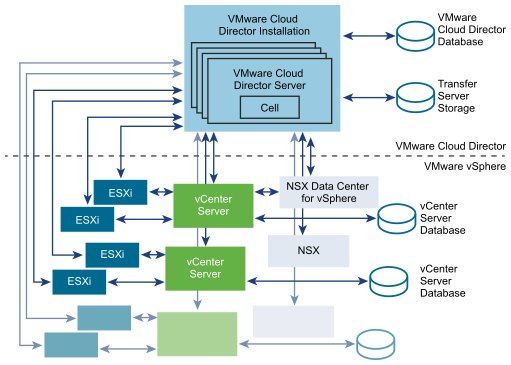
\includegraphics[scale=0.7]{figures/vcloud_components.png}
	\caption{اجزای تشکیل دهنده \lr{vCloud}\cite{mstoimenova}}
	\label{fig:vcloud_components}
\end{figure}

مهم‌ترین مولفه‌ی تشکیل‌دهنده، خدمت‌گزار \lr{vCenter} است که وظیفه‌ی مدیریت منابع مجازی در مرکزداده را بر عهده دارد. خدمت‌گزار \lr{vCenter} با فراناظر\LTRfootnote{Hypervisor} \lr{vSphere} ارتباط برقرار می‌کند تا عملیات کلیدی مانند ایجاد، استقرار و مدیریت ماشین‌ها و منابع مجازی را انجام دهد.

مولفه دیگر که برای مجازی‌سازی خدمات شبکه طراحی شده‌است، سکوی \lr{NSX} است که وظیفه‌ی ارائه‌ی قابلیت‌های مجازی‌سازی شبکه به مرکزداده را بر عهده دارد. \lr{NSX} مجازی‌سازی شبکه را با ایجاد شبکه‌های ایزوله از یکدیگر فراهم می‌کند و به چندین مستأجر\LTRfootnote{Tenant} اجازه می‌دهد تا زیرساخت فیزیکی مشابهی را بدون تداخل با یک‌دیگر به اشتراک بگذارند.

مولفه‌ی مجازی‌سازی‌ خدمات ذخیره‌سازی دائم، توسط \lr{vSAN} ارائه شده‌است که یک سکو‌ی  ذخیره‌سازی نرم‌افزاری است که مشتریان را قادر می‌سازد منابع ذخیره‌سازی را در یک محیط مجازی مدیریت کنند. \lr{vSAN} به مشتریان امکان ایجاد حجم\LTRfootnote{Volume}‌های ذخیره‌سازی مجازی را می‌دهد که می‌تواند برای ذخیره‌ی فایل‌های ماشین مجازی و همچنین فضای ذخیره‌ی اشیا\LTRfootnote{Object Storage} استفاده شود.

در نهایت، سکو‌ی \lr{VMWare Cloud Director} یک رابط برنامه‌نویسی ارائه می‌کند که به مشتریان اجازه می‌دهد زیرساخت ابری خود را مدیریت کنند. این رابط برنامه‌نویسی بر پایه‌ی استاندارد \lr{REST} تعریف شده که می‌تواند برای عملیات‌ مختلف مانند ایجاد و مدیریت ماشین‌های مجازی، شبکه‌ها و حجم‌های ذخیره‌سازی استفاده شود.

\section{زبان برنامه‌نویسی}
برای پیاده‌سازی سامانه‌ی مورد نظر باید از یک زبان برنامه‌نویسی وب استفاده کنیم. با توجه به حجم بالای درخواست‌ها و فشار بر روی خدمت‌گزار، سرعت زیاد و حجم و پیچیدگی کم در منطق سامانه، از معیار‌های کلیدی انتخاب زبان برنامه‌نویسی است. یکی دیگر از این معیارها، محبوبیت و توسعه‌پذیری زبان برنامه‌نویسی در آینده برای نیازمندی‌های احتمالی و پیش‌بینی نشده است. با توجه به این معیارها، انتخاب ما برای توسعه‌ی این پروژه، زبان برنامه‌نویسی \lr{Go} است.

\subsection{زبان برنامه‌نویسی \lr{Go}}
زبان \lr{Go} یک زبان برنامه‌نویسی تابعی\LTRfootnote{Functional} است که با گذر زمان محبوبیت زیادی کسب کرده و توسط بسیاری از شرکت‌ها و توسعه‌دهندگان برای ساخت برنامه‌های کاربردی مقیاس‌پذیر\LTRfootnote{Scalable} استفاده می‌شود. این زبان برای توسعه‌ی ‌یک سرویس جامع ارائه‌ی خدمات \lr{IaaS}، مزیت‌های قابل توجه و همچنین معایبی دارد که در ادامه به شرح دقیق‌تر آن‌ها می‌پردازیم.

\clearpage

مزایای استفاده از \lr{Go} برای پیاده‌سازی یک رابط برنامه‌نویسی مقیاس‌پذیر شامل این موارد اس\cite{Lockard2019}:
\begin{enumerate}

\item  \textbf{هم‌زمانی\LTRfootnote{Concurrency} به صورت ذاتی}: یکی از برجسته‌ترین مزایای \lr{Go}، پشتیبانی قوی آن در مدیریت همزمانی است که آن را برای ساختن سیستم‌های بزرگ‌مقیاس که نیاز به استفاده‌ی کارآمد از منابع دارند، مناسب می‌کند. در یک محیط ابری که تقاضا برای منابع می‌تواند به سرعت تغییر کند، مدل پیاده‌سازی هم‌زمانی در \lr{Go}، به‌کارگیری منابع را در حالتی ایده‌آل حفظ می‌کند.


\item  \textbf{مدیریت حافظه}: \lr{Go} دارای یک جمع‌کننده زباله\LTRfootnote{Garbage Collector} داخلی است که مدیریت حافظه را آسان‌تر می‌کند و بر خلاف زبان‌های سطح پایین مانند \lr{C} و \lr{C++} این فرصت را به توسعه‌دهندگان می‌دهد تا روی عملکرد برنامه‌شان تمرکز کنند. این مورد همچنین به کاهش خطر نشت حافظه\LTRfootnote{Memory Leak} کمک می‌کند، که می‌تواند باعث ایجاد مشکلات پایداری و امنیتی شود.

\item \textbf{سادگی}: \lr{Go} دارای یک نحو\LTRfootnote{Syntax} ساده و شبیه به زبان‌های بسیار معروف \lr{C}و پایتون است که یادگیری و استفاده از آن را نسبت به زبان‌های دیگر برنامه‌نویسی آسان‌تر می‌کند.

\item \textbf{کارایی\LTRfootnote{Performance}}: \lr{Go} برای کارایی بهینه طراحی شده‌است. برای سامانه‌ها و برنامه‌هایی که باید بار پویا و در مقیاس بالا را مدیریت کنند، یک گزینه مناسب محسوب می‌شود. کامپایل شدن برنامه‌ها و اجرای مستقیم بر روی سیستم عامل در کنار  محیط اجرای بهینه، این زبان برنامه‌نویسی را از نظر زمان اجرا در کنار زبان‌های سطح پایینی همچون \lr{C++} قرار می‌دهد.\cite{Donovan2015}
\end{enumerate}

با وجود این مزیت‌ها، چالش‌هایی نیز برای استفاده از این زبان برنامه‌نویسی مطرح اس\cite{Lockard2019}. از جمله:
\begin{enumerate}
\item \textbf{محدود بودن جامعه}: باوجود محبوبیت رو به رشد این زبان برنامه‌نویسی، به دلیل سن کم‌تر نسبت به زبان‌های دیگر مانند \lr{JavaScript}، \lr{Java} و یا \lr{Python}، این زبان برنامه‌نویسی از جامعه‌ی متن‌باز کوچک‌تری برخوردار است که به سبب آن محدودیت‌هایی برای کتاب‌خانه‌ها و قطعه کد‌های خاص‌منظوره پدیدار شده است.

\item \textbf{شیب یادگیری تند}: با وجود نحو آشنا و نزدیک \lr{Go}، این زبان از اصول و ضرب‌المثل\LTRfootnote{Idiom}‌های خاصی پیروی می‌کند که ممکن است در چهارچوب‌ها و الگوهای زبان‌های دیگر حضور نداشته باشند. توسعه‌ی برنامه‌های شاخص و الگو، نیازمند رعایت این اصول است که این امر، اثرگذاری افراد با تجربه‌ی کم در توسعه‌ی برنامه‌های این زبان را کاهش می‌دهد.
\end{enumerate}

با وجود این مسائل از بین گزینه‌های موجود، انتخاب نهایی ما زبان برنامه‌نویسی \lr{Go} است.

\section{استاندارد \lr{REST}}
در تمام برنامه‌های تحت وب، یکی از کلیدی‌ترین تصمیمات در طراحی، انتخاب پروتکل و استاندارد‌های مربوط به انتقال داده و اتصال برنامه‌ به کاربر است. یکی از پرکاربردترین استانداردهای مورد استفاده در برنامه‌های تحت وب، استاندارد \lr{REST}\LTRfootnote{Representational State Transfer} است.

عملیات محدود و وجود قوانین جامع، باعث سادگی تعریف و توسعه‌ی نقطه‌های دسترسی به منابع با این استاندارد شده‌است. همچنین عدم نگهداری وضعیت بین درخواست‌ها باعث می‌شود که به سادگی بتوان برنامه‌ها را به صورت افقی نسبت به بار مقیاس کرد. با توجه به اینکه قوانین در این استاندارد کاملا مستقل از زیرساخت و سکوی توسعه و اجرا است، استفاده از این استاندارد، امکان استفاده‌ی گستره‌ی بسیار وسیعی از کاربران از خدمات را فراهم می‌آورد.\cite{Fielding:2000}

همچنین زبان \lr{Go} به صورت طبیعی از این استانداردها پیروی می‌کند و کتاب‌خانه و چهارچوب‌های متعددی از جمله چهارچوب \lr{Echo} برای این منظور در جامعه‌ی متن‌باز این زبان، یافت می‌شود.

\section{پایگاه ذخیره داده}
برنامه‌ی ما نیازمند ذخیره‌سازی طیف گسترده‌ای از اطلاعات است. این اطلاعات شامل تنظیمات و اطلاعات مورد نیاز هر بخش از سامانه، رخداد‌ها و وقایع رخ داده در سامانه و منابع و مدل‌های مورد استفاده‌ی کاربران می‌شود. برای ذخیره‌سازی این اطلاعات، انتخاب‌های متعددی برای پایگاه داده داریم که در این پروژه بسته به ماهیت داده و نوع وابستگی برنامه به آن، از دو دسته‌ی کلی پایگاه‌های داده رابطه‌ای و غیر رابطه‌ای استفاده می‌کنیم.

\subsection{پایگاه داده رابطه‌ای}
پایگاه داده‌های رابطه‌ای، به دسته‌ای از پایگاه‌های داده گفته می‌شود که بر مبنای زبان پرسمان ساختاریافته (\lr{SQL}\LTRfootnote{Structured Query Language}) تعریف شده‌اند. در این پایگاه‌های داده، اطلاعات در جداولی با روابط تعریف‌شده، سازماندهی می‌شوند و پرسمان‌ها را می‌توان با استفاده از \lr{SQL} برای بازیابی داده‌های خاص ایجاد کرد. نمونه‌هایی از پایگاه داده‌های \lr{SQL} عبارتند از \lr{MySQL}، \lr{Oracle} و \lr{Microsoft SQL Server}. پایگاه‌های داده‌ی \lr{SQL} برای برنامه‌هایی که نیاز به تراکنش‌های پیچیده دارند و شامل مقادیر زیادی از \textbf{داده‌های ساختاریافته} هستند؛ مانند سیستم‌های مالی، سامانه‌های مدیریت کاربران و تعریف منابع با قابلبیت تغییر مکرر مناسب هستند.


به طور کلی، اطلاعات ساختاریافته‌ای را که می‌‌توان در جداول با ستون‌های ثابت تعریف کرد، در این پایگاه داده ذخیره می‌کنیم. در این پروژه، ما از پایگاه داده‌ی \lr{\textbf{PostgreSQL}} که یکی از معروف‌ترین پایگاه داده‌های رابطه‌ای متن‌باز است استفاده می‌کنیم. 
\subsection{پایگاه داده غیر‌ رابطه‌ای}
در مقابل پایگاه‌ داده‌های رابطه‌ای، پایگاه داده‌های غیر رابطه‌ای (\lr{NoSQL}\LTRfootnote{Not Only SQL}) تعریف می‌شوند. این دسته از پایگاه‌های داده به گونه‌ای طراحی شده ‌اند که بتوانند حجم بسیار زیادی از اطلاعات نیمه ساختار یافته\LTRfootnote{Semi Structured Data} را پردازش کنند. این اطلاعات همانگونه که از مفهومش برداشت می‌شود ساختار ثابت و جدول مانند ندارد، بلکه حالت‌های متنوعی از جمله کلید-مقدار، سند پایه، گراف پایه و ستون پایه را شامل می‌شود\cite{Stonebraker2010}.

در این پروژه ما رخدادهای سامانه که ساختار یکتایی ندارند و همچنین از حجم بسیار بالایی برخوردار هستند را در پایگاه داده غیر رابطه ای ذخیره می‌کنیم. ابزاری که برای این منظور استفاده می‌کنیم پایگاه داده‌ی \lr{\textbf{MongoDB}} است که یک پایگاه داده‌ی متن‌باز است.

\section{معماری میکروسرویس}
معماری میکروسرویس\LTRfootnote{Microservice} یک الگوی طراحی\LTRfootnote{Design Pattern} محبوب است که در توسعه‌ی نرم‌افزار‌های مدرن برای ایجاد برنامه‌های کاربردی مقیاس‌پذیر، قابل نگهداری و انعطاف‌پذیر استفاده می‌شود. این معماری بر اساس ایده‌ی تجزیه‌ی یک سیستم نرم‌افزاری پیچیده به سرویس‌های کوچکتر و مستقل است که می‌توانند به طور مستقل، توسعه یافته، استقرار یابند و مدیریت شوند. این رویکرد چندین مزیت از جمله بهبود مقیاس‌پذیری، افزایش تحمل خطا و سرعت توسعه را ارائه می‌دهد.

میکروسرویس مبتنی بر مفهوم معماری سرویس‌گرا (\lr{SOA}\LTRfootnote{Service-Oriented Architecture}) است که شامل تجزیه‌ی یک سیستم نرم‌افزاری پیچیده به اجزای کوچکتر و مستقل است. با این حال، معماری میکروسرویس، این مفهوم را با تعریف هر مؤلفه به عنوان یک سرویس جداگانه که برای انجام یک عملکرد واحد طراحی شده است، یک قدم جلوتر می‌برد. این رویکرد به درجه بسیار بالاتری از انعطاف‌پذیری منجر می‌شود، زیرا هر سرویس می‌تواند مستقل از سایر سرویس‌ها مدیریت و دچار دخل و تصرف شود.

بخشی از مزایای این معماری در برنامه‌های داده‌محور\LTRfootnote{Data Driven} و رخداد‌محور \LTRfootnote{Event Driven} در زیر توضیح داده شده\cite{Hightower2017}\cite{Fowler2014}:
\begin{itemize}
\item \textbf{سرعت توسعه نرم‌افزار}: با توجه به مستقل بودن واحد‌های تعریف‌شده‌ی برنامه در این معماری، تیم‌ها و افراد مختلف می‌توانند مستقل و موازی بر توسعه سامانه کار کنند. این امر باعث افزایش قابل توجه سرعت و چابکی توسعه برنامه‌ها می‌شود. همچنین با توجه به تعریف روابط میان سرویس‌ها از قبل، اعمال و اجرای تغییرات درونی برنامه‌ها بسیار راحت‌تر و سریع‌تر انجام می‌شود.

\item \textbf{مقیاس پذیری}: به دلیل جدا و منزوی بودن سرویس‌ها در این معماری، مقیاس هر سرویس را می‌توان متناسب با بار سامانه تنظیم کرد. این مورد به این معنی است که می‌توان قسمت‌های مختلف سامانه را در هر زمان کم و زیاد یا بزرگ و کوچک کرد.

\item \textbf{تحمل خطا}: هرگونه خطا و اخلال در یک سرویس در معماری میکروسرویس، از قبل پیش‌بینی شده است و همواره می‌توان تمهیدات لازم جهت تحمل خطا را در سرویس‌های دیگر از پیش آماده کرد. همچنین اخلال در یک سرویس، فقط در همان سرویس اثرگذار است و عملکرد سایر سرویس‌های مستقل دچار اختلال نمی‌شود.

\end{itemize}

با وجود این مزایا، این معماری چالش‌ها و معایبی را نیز به دنبال دارد\cite{Hightower2017}\cite{Fowler2014} که در ادامه به بررسی آنها می‌پردازیم.

\begin{itemize}
	 \item \textbf{پیچیدگی طراحی}: هنگام طراحی میکروسرویس‌های موجود در یک سامانه، باید تمامی روابط و هماهنگی‌های میان‌سرویسی را از قبل تعریف کرد. هرگونه خطا و کاستی در این مرحله، منجر به چالش‌های اساسی در مرحله اجرا و توسعه می‌شود که برطرف کردن آنها نیازمند هزینه‌ی بیشتری است. پس باید نهایت دقت را در مرحله طراحی میکروسرویس‌ها به خرج داد.
	
	 \item \textbf{زیرساخت}: اجرا و پیاده‌سازی میکروسرویس‌ها نیازمند پیش‌نیاز‌ها و زیرساخت‌های خاص و ابزار‌های متعدد است که هزینه استفاده از این معماری را برای برنامه‌هایی با مقیاس کم و دامنه امکانات محدود، زیاد می‌کند. نیاز این معماری به تضمین زیرساخت اجرایی و شبکه‌ای از جمله‌ی این پیش‌نیازها است.
	
	 \item \textbf{حفظ سازگاری داده}\LTRfootnote{Data Consistency}: با گسترده شدن داده‌ها میان سرویس‌های مختلف و احتمال وجود خطا در هر قسم\LTRfootnote{Partition} از سامانه، تضمین سازگاری داده بدون ضمانت سلامت زیرساخت امری بسیار دشوار است.
	
	 \item \textbf{سربارهای اضافی}: استفاده از سرویس‌های متعدد برای سامانه‌ها با دامنه فعالیت‌های محدود، باعث به‌وجود آمدن سربار‌های کد، شبکه و محاسبات می‌شود.
\end{itemize}

در نهایت، براساس موارد مطرح شده، برای تصمیم‌گیری در مورد استفاده از معماری میکروسرویس، باید دامنه‌ی فعالیت‌ها، فشار ناشی از بار در قسمت‌های مختلف، محدودیت‌های تیم توسعه و محدودیت‌های زیرساخت سامانه را در نظر گرفت. با در نظر گرفتن این موارد، در این پروژه معماری مورد استفاده‌ی ما، معماری میکروسرویس است.

\section{‌دروازه‌ی ورود رابط}
الگوی طراحی ‌دروازه‌ی ورود رابط\LTRfootnote{API Gateway}، یکی از الگوهای رایجی است که در کنار میکروسرویس‌ها استفاده می‌شود. در این الگو، برنامه‌ای به عنوان یک پیش‌کار\LTRfootnote{Proxy} که وظیفه‌ی مسیریابی درخواست‌های ورودی را بر عهده دارد، قرار داده می‌شود. مدیریت بخش بزرگی از موارد امنیتی، نظارتی و سلامتی میکروسرویس‌ها بر عهده این لایه قرار می‌گیرد.

در حالت پیش‌فرض شکل\ref{fig:no-api-gateway}، کاربران سامانه مستقیما با میکروسرویس‌ها در ارتباط هستند که این امر ملاحظات جدی امنیتی و کارایی به دنبال دارد. در این حالت، تمامی میکروسرویس‌ها باید عملیات مشترکی همچون احراز هویت، واقعه‌نگاری ونظارت را پیاده‌سازی کنند.


\begin{figure}[h]
	\vspace{1cm}
	\centering
	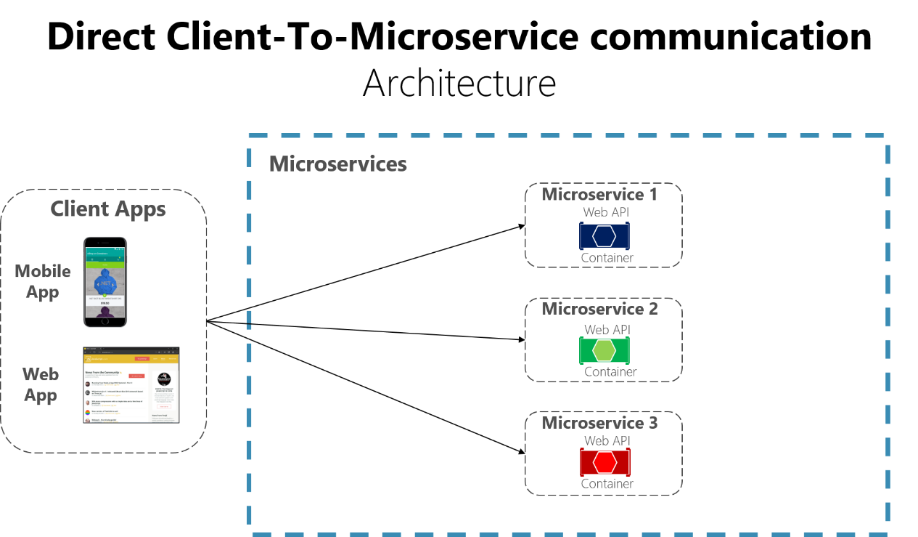
\includegraphics[scale=1.4]{figures/direct-client-to-microservice-communication.png}
	\caption{معماری یک سامانه میکروسرویس بدون ‌دروازه‌ی ورود رابط\cite{Microsoft_API_Gateway_2023}}
	\label{fig:no-api-gateway}
\end{figure}

در مقابل معماری شکل\ref{fig:no-api-gateway}، معماری سامانه در صورت استفاده از یک دروازه‌ی ورود رابط، مانند شکل\ref{fig:api-gateway} می‌شود. در این معماری، تعداد قابل توجهی از عملیات مشترک را می‌توان در لایه ‌دروازه‌ی ورود انجام داد. به طور کلی، مزیت‌های استفاده از ‌دروازه‌ی ورود رابط را می‌توان به شکل زیر بیان کرد\cite{Microsoft_API_Gateway_2023}:

\begin{itemize}
	\item \textbf{مدیریت متمرکز}: هنگامی که دروازه‌ی مکاتبه و تعامل با تمامی کاربران سامانه ثابت و مشخص باشد، مدیریت نحوه‌ی این ارتباط کاملا مستقل از عملکرد درونی سامانه می‌شود و می‌توان نظارت و مدیریت کامل‌تری بر روی درخواست‌های کاربران و پاسخگویی به آن‌ها داشت.
	
	\item \textbf{امنیت}: با وجود یک لایه‌ی کاملا مستقل در پیش‌روی کاربر، می‌توان مکانیزم‌های امنیتی نظیر احراز هویت و مجوزها را در کنار موارد امنیت شبکه یکجا مدیریت کرد. این گونه میکروسرویس‌ها، کاملا درون یک شبکه منزوی و غیر قابل دسترس از بیرون تجمیع می‌شوند که خطر ریسک‌های امنیتی را به شکل قابل توجهی کاهش می‌دهد.
	
	\item \textbf{تقسیم بار}: لایه ‌دروازه‌ی ورود می‌تواند بار ورودی را بین نسخه‌های متعدد میکروسرویس‌ها تقسیم کند و در صورت نیاز اتصال به بخش‌های خاصی از سامانه را کمتر یا زیادتر کند.
	
\item \textbf{نظارت}: با پیاده‌سازی واحدهای نظارتی در ‌دروازه‌ی ورود، تمامی رفتار کاربران و نحوه برخورد‌ سامانه با آن‌ها را یکجا و به ‌طور متمرکز در اختیار خواهیم داشت که برای مقاصد ایرادیابی و تحلیلی فواید زیادی دارد.
\end{itemize}

\begin{figure}[h]
	\vspace{1cm}
	\centering
	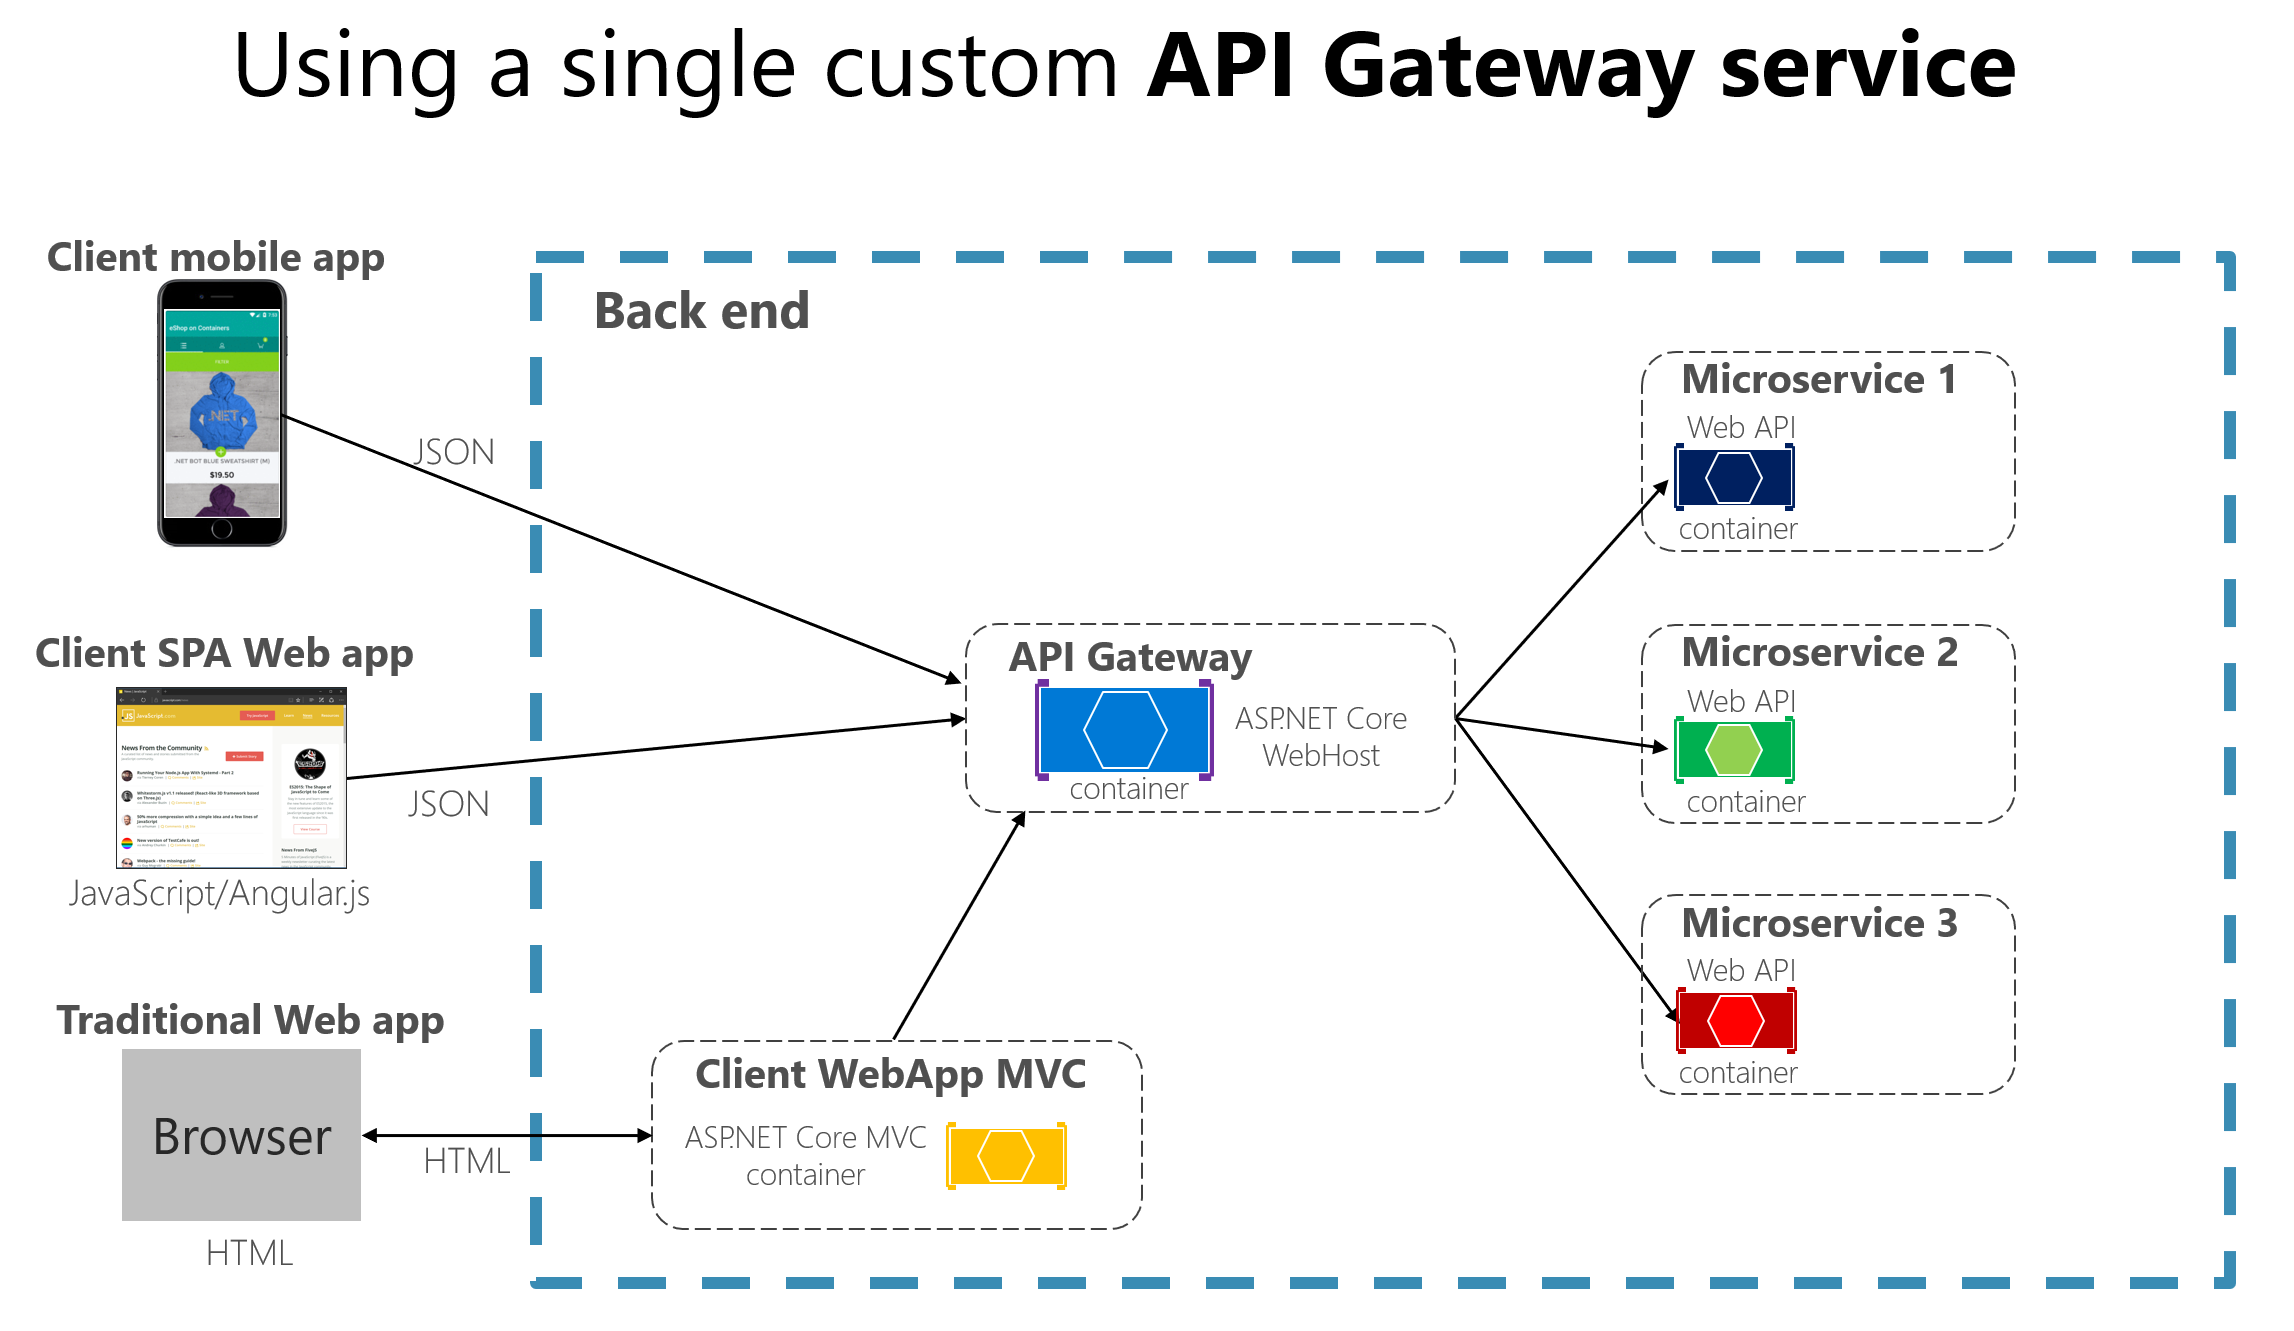
\includegraphics[scale=0.5]{figures/custom-service-api-gateway.png}
	\caption{معماری یک سامانه میکروسرویس با وجود یک ‌دروازه‌ی ورود رابط\cite{Microsoft_API_Gateway_2023}}
	\label{fig:api-gateway}
\end{figure}

\section{داکر}
داکر\LTRfootnote{Docker} یکی از کاربردی‌ترین ابزار‌ها برای پیاده‌سازی معماری میکروسرویس است. این ابزار که خود از چندین بخش تشکیل شده، امکان بسته‌بندی برنامه‌ها در واحد ظرف اجرایی\LTRfootnote{Container} را فراهم می‌کند و کاربران می‌توانند این ظروف اجرایی را در یک موتور ظرف اجرایی\LTRfootnote{Container Engine} مثل موتور داکر\LTRfootnote{Docker Engine} اجرا کنند. با انجام این کار، ظرف اجراییها به صورت مستقل از یکدیگر در یک محیط منزوی اجرا می‌شوند. فواید این مدل اجرا، شامل مقیاس پذیری راحت، قابل حمل بودن واحد‌های اجرایی برنامه، سازگاری و انعطاف پذیری نسبت به محیط اجرا و ابزار‌ها است. معماری کلی داکر و فرایند عملکرد این ابزار در شکل\ref{fig:docker-arch} مشخص شده است. کاربران با استفاده از برنامه \lr{docker} 
با سرویس \lr{docker daemon} که همواره در پس‌زمینه در‌حال اجرا است، در تعامل‌ خواهند بود. این برنامه سپس تصاویر\LTRfootnote{Images} را از مخزن محلی و یا مرکزی دریافت کرده و در قالب ظرف اجراییهای موتور داکر اجرا‌ می‌کند.
\begin{figure}[h]
	\vspace{1cm}
	\centering
	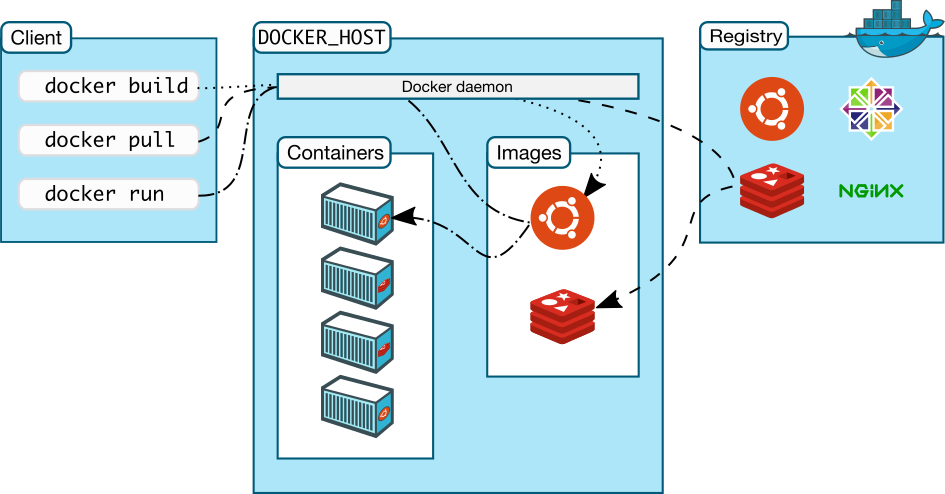
\includegraphics[scale=0.4]{figures/docker-architecture.png}
	\caption{معماری داکر}
	\label{fig:docker-arch}
\end{figure}

تفاوت ظرف اجراییهای داکر با ماشین‌های مجازی که در گذشته به همین منظور استفاده می‌شدند در شکل\ref{fig:docker-container-vm}‌ قرار گرفته‌است. برخلاف ماشین مجازی، ظرف اجراییها توسط موتور ظرف اجرایی (در این شکل موتور داکر) بر روی سیستم عامل میزبان اجرا می‌شوند. این مدل اجرا، باعث از بین  رفتن سربارهای مجازی سازی دستورات و سخت افزار می‌شود.

\begin{figure}[h]
	\vspace{1cm}
	\centering
	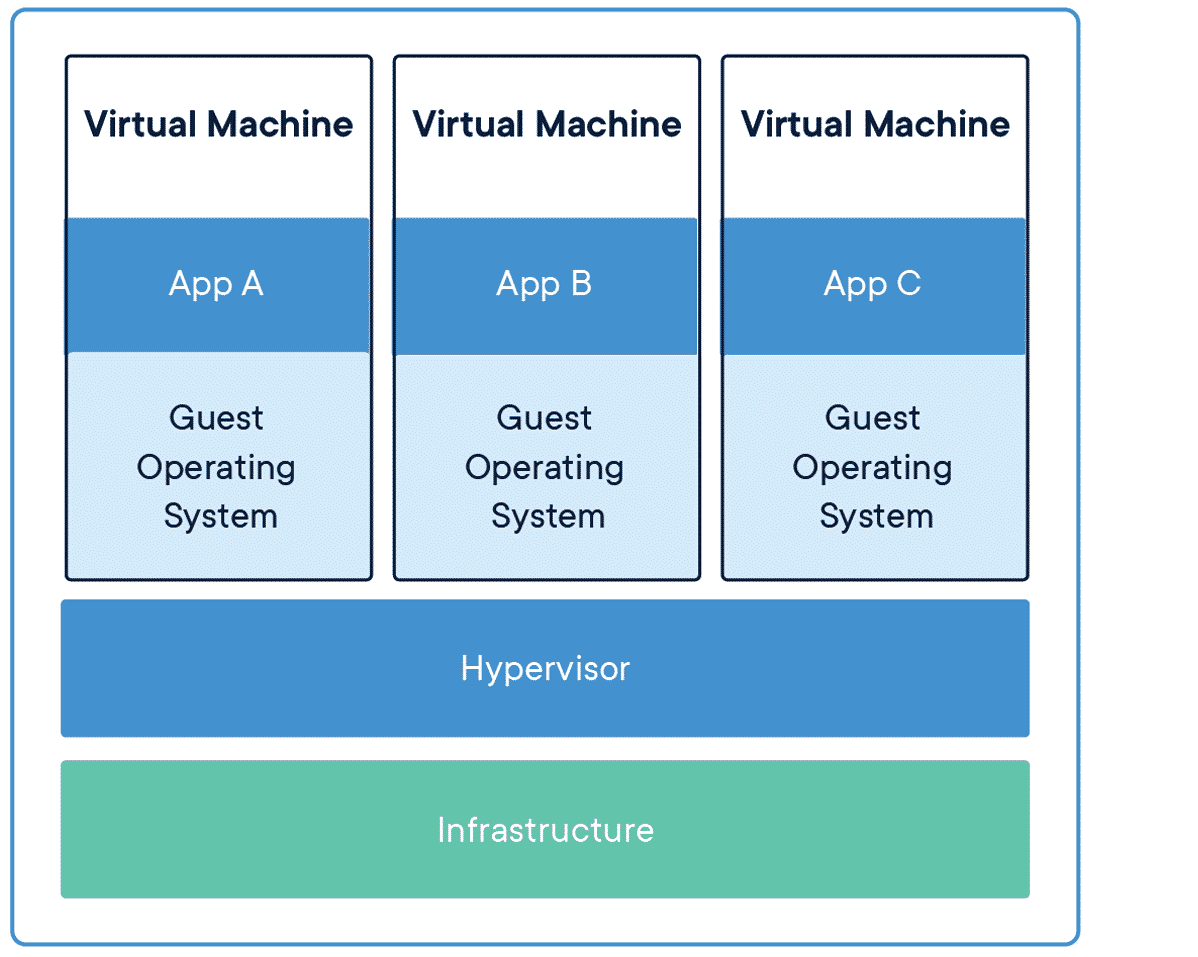
\includegraphics[scale=0.17]{figures/container-vm-whatcontainer.png}
	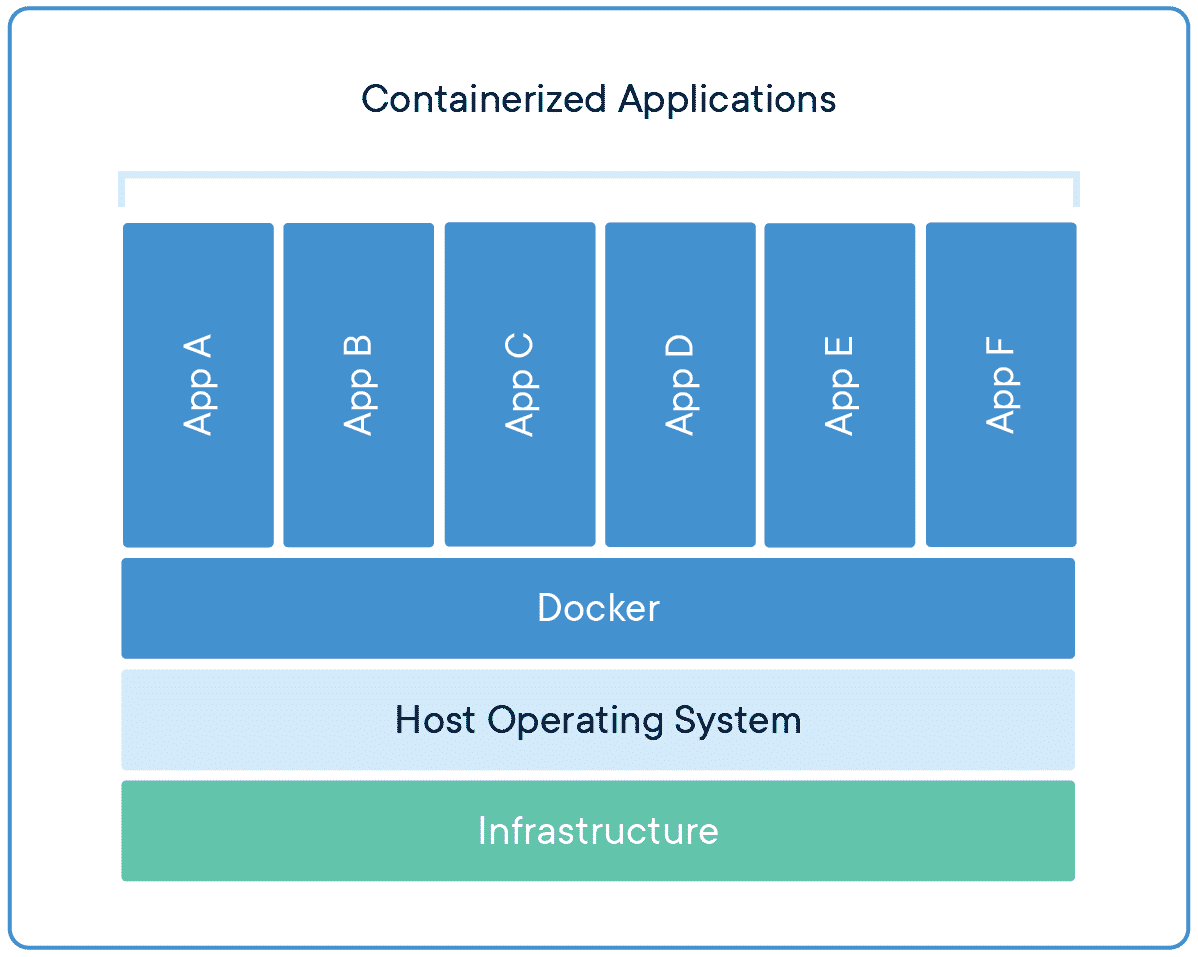
\includegraphics[scale=0.17]{figures/docker-containerized-appliction-blue-border.png}
	\caption{لایه‌های ظرف اجرایی داکر}
	\label{fig:docker-container-vm}
\end{figure}


\section{نتیجه گیری}

در این پروژه، ما به عنوان زیرساخت ارائه خدمات \lr{IaaS} از سرویس \lr{VMWare Cloud Director} بهره گرفتیم. برای سرویس‌های مورد نیاز برای توسعه خدمات، از زبان برنامه‌نویسی \lr{Go} و از چهارچوب‌ها و کتاب‌خانه‌های این زبان استفاده کردیم. رابط‌های سامانه با کاربران بیرون و تعاملات درونی سامانه از استاندارد \lr{REST} پیروی می‌کنند و کتاب‌خانه \lr{Echo} در زبان برنامه‌نویسی \lr{Go} برای پیاده‌سازی این موضوع به کار گرفته شده‌است. برای ذخیره داده از فناوری‌های پایگاه داده رابطه‌ای و غیر رابطه‌ای استفاده کردیم. راه اندازی پایگاه داده رابطه‌ای با ابزار \lr{PostgreSQL} است و برای پایگاه داده غیر رابطه‌ای از ابزار \lr{MongoDB} استفاده کرده‌ایم.

پیاده‌سازی سرویس‌ها در قالب معماری میکروسرویس انجام‌شد که تمامی قسمت‌های سامانه در قالب تصاویر داکر قرار گرفتند. این سرویس‌ها داخل یک شبکه داخلی پشت یک ‌دروازه‌ی ورود رابط جای گرفتند که این ‌دروازه‌ی ورود رابط، وظیفه‌های نظارت، احراز هویت و ثبت وقایع را برعهده دارد.